\documentclass[a4paper, 12pt]{article}

% Packages
\usepackage[german]{babel}
\usepackage[top=4cm, bottom=2cm, left=4cm, right=2cm]{geometry}
\usepackage[utf8]{inputenc}
\usepackage{apacite}
\usepackage{fancyhdr}
\usepackage{caption}
\usepackage{graphicx}
\usepackage{url}
\usepackage{pdfpages}
\usepackage{setspace}
\usepackage{tabulary}
\usepackage[multiple]{footmisc}
%\usepackage[hidelinks]{hyperref}

% Layout Einstellungen
%% Seitennummerierung oben mitte ohne durchgezogene Linie
\pagestyle{fancy}
\setlength{\headheight}{15pt}
\renewcommand\headrulewidth{0pt}
\chead{\thepage}
\lhead{}
\rhead{}
\lfoot{}
\cfoot{}
\rfoot{}
%% Zeilenabstand
\linespread{1.5}%\selectfont
%\onehalfspacing
%% Zeilenformatierung
%\fussy%
\sloppy
%% Abstand zwischen Absätzen
\setlength{\parskip}{2ex plus0.5ex minus0.5ex}
%% Keine Einrückung von Absätzen
\setlength{\parindent}{0em}
\bibliographystyle{apacite}

\begin{document}
	\includepdf{pdf/title.pdf}
	\pagenumbering{Roman}
	\setcounter{page}{2}
	\tableofcontents
%	\listoffigures
%	\listoftables
	\clearpage
	\pagenumbering{arabic}
	\section{Einleitung}
Die wissenschaftliche Forschung wurde als wichtiger Einflussfaktor für die Entstehung neuer Technologien und Technologietrends in bedeutenden Studien nachgewiesen.\footnote{\citeNP<Vgl.>[S.~187]{Nelson1986}.}\footnote{\citeNP<Vgl.>[S.~11]{Mansfield1991}.}\footnote{\citeNP<Vgl.>[S.~599]{Tegarden2012}.}
Nach Jaffe wird diese Erkenntnis bereits durch die geographische Nähe von Zentren der Spitzentechnologie wie das "`Silicon Valley"' oder die "`Massachusetts Route 128"' zu führenden Universitäten gestützt.\footnote{Vgl. \citeNP{Jaffe1989}, S.~967f.} Nach einer Studie von Mansfield wären etwa 11~\% aller Produkte einer Auswahl aus sieben Fertigungsindustrien im Betrachtungszeitraum gar nicht oder nur mit erheblicher Zeitverzögerung entwickelt worden, wäre dem nicht eine entsprechende wissenschaftliche Forschung vorausgegangen.\footnote{\citeNP<Vgl.>[S.~2]{Mansfield1991}.}

Dennoch liegt die maßgebliche Entscheidung über den Einsatz und die Weiterentwicklung neuer Technologien vorwiegend in Händen von Unternehmern, Managern und sonstigen Entscheidungsträgern der praktizierenden Wirtschaft. Die wiederum richten ihre Entscheidungen unter Berücksichtigung einer Vielzahl von Faktoren an den Markt aus, um den Unternehmenserfolg zu steigern.\footnote{Vgl. \citeNP{Gruber2008}, S.~1652f.} Dabei greifen sie auch auf Informationsquellen von spezialisierten Unternehmen zurück, die mit Hilfe proprietärer Methoden Prognosen für Technologietrends in eigenen Publikationen herausgeben. Einer der einflussreichsten und bekanntesten Vertreter dessen ist der "`Gartner Hype Cycle"', den große Unternehmen bei strategischen Entscheidungen bezüglich neuer Technologien beratend hinzuziehen.\footnote{\citeNP<Vgl.>[S.~254]{Steinert2010}.}

Nach Beyer ist der Einfluss auf Technologietrends durch Wirtschaftsmedien höher als durch wissenschaftliche Artikel, da sie von Managern aufgrund des gewohnten Fachjargons sowie der Praxisrelevanz bevorzugt gelesen werden.\footnote{Vgl. \citeNP{Beyer1992}, S.~472.} Barley et al. fanden sogar heraus, dass sich gängige Begriffe der Wirtschaft in wissenschaftlicher Literatur verzögert manifestieren, folglich der Einfluss unidirektional von Unternehmern in Richtung Akademiker stattfindet.\footnote{Vgl. \citeNP{Barley1988}, S.~52.} Nach Spell hängt das allerdings eher damit zusammen, dass wissenschaftliche Artikel einem Peer-Review unterzogen werden, welcher Monate bis Jahre in Anspruch nehmen kann, bis sie in Fachartikeln erscheinen, als dass wissenschaftliche Forschungsschwerpunkte stets aus Wirtschaftsjournalen gespeist würden.\footnote{Vgl. \citeNP{Spell1999}, S.~345.}

\subsection{Problemstellung}
Somit findet eine gegenseitige Einflussnahme hinsichtlich der Prognose von Technologietrends zwischen Entscheidungsträgern der Wirtschaft und akademischen Forschern zweifelsohne statt. Gleichzeitig ist aufgrund teils unterschiedlicher Interessen beider Parteien eine Diskrepanz bei der Schwerpunktsetzung evident. 

Technologiethemen insbesondere in Informationstechnologien sind ständiger Ver\-änderung unterworfen\footnote{Vgl. \citeNP{Chang2009}, S.~107f.}, wodurch eine permanente Auseinandersetzung mit Trend\-themen für beide Seiten unumgänglich ist. Obwohl das "`Gartner Hype Cycle"' bei der Lösung dieser Herausforderung hohe Anerkennung in der Praxis genießt, bleibt es in der akademischen Forschung weitestgehend unberücksichtigt.\footnote{Vgl. \citeNP{OLeary2008}, S.~241.}\footnote{Vgl. \citeNP{Jarvenpaa2008}, S.~12.}

Folglich stellt sich die Frage, ob und in welchem Ausmaß sich prognostizierte Technologietrends aus der wirtschaftlichen Praxis in wissenschaftlichen Fachartikel widerspiegeln.

\subsection{Zielsetzung}
Das vorrangige Ziel der Arbeit ist es, über einen definierten Zeitraum Technologiethemen mit der höchsten medialen Präsenz in der Wirtschaft zu erfassen und die Verteilung dieser Themen in wissenschaftlichen Fachartikeln im Verhältnis gegenüberzustellen.

Dazu wird eine Datenbasis der Trendthemen aus dem "`Gartner Hype Cycle for Emerging Technologies"' für die jeweiligen Jahre des ausgewählten Zeitraumes entnommen. Anschließend werden diese Daten in mehreren Datenbanken für wissenschaftliche Fachartikel im vergleichbaren Zeitraum gesucht, um sie schließlich mit Hilfe quantitativer Methoden miteinander zu vergleichen.

Als Ergebnis der Analyse wird die Erkenntnis angestrebt, mögliche Diskrepanzen beim Verständnis für vielversprechende Trends festzustellen.

\subsection{Leitfragen}
Die einleitend genannte Feststellung, dass sich akademische Forschungsschwerpunkte im Bereich von neuen Technologien mit zeitlicher Verzögerung zur wirtschaftlichen Praxis etablieren, ist zum Ende des letzten Jahrhunderts gemacht worden. Der "`Gartner Hype Cycle"' ist etwa zur gleichen Zeit erstmalig im Jahre 1995 erschienen\footnote{Vgl. \citeNP{OLeary2008}, S.~241.} und findet folglich in diesen Artikeln keine Berücksichtigung.

Um die Aktualität dieser Erkenntnis zu eruieren, werden hieraus folgende Leitfragen abgeleitet:

\begin{description}
	\item[L1:] Wie ist das Verhältnis zwischen Technologien im Abschnitt "`Peak of Inflated Expectations"' und der Anzahl an wissenschaftlichen Publikationen im vergleichbaren Zeitraum?
\end{description}

\begin{description}
	\item[L2:] Ist eine erstmalig erschienene Technologie des "`Gartner Hype Cycle"' im Ab\-schnitt "`Peak of Inflated Expectations"' in wissen\-schaftlichen Ver\-öf\-fent\-lichungen als Trend wahrzunehmen?
\end{description}

\begin{description}
	\item[L3:] Wenn eine Technologie in einer späteren Ausgabe des "`Hype Cycle"' herausfällt, steigt die Anzahl wissenschaftlicher Artikel um eine gewisse Zeit weiter, bis sie stagniert bzw. abnimmt?
\end{description}

Durch die retrospektive Analyse vergangener Trendthemen können mit heutiger Betrachtung möglicherweise weitere Leitfragen hinsichtlich der Ursachen für Abweichungen aufgestellt werden, die als Grundlage für die weitere Forschung dienen können.

\subsection{Methodik}
Wegen der eingangs erwähnten Relevanz wird der "`Gartner Hype Cycle for Emerging Technologies"' als Stellvertreter für die wirtschaftliche Praxis bei der Bestimmung kommender Trendthemen angenommen. Dabei handelt es sich um die graphische Darstellung des üblicherweise zu beobachtenden Reifeprozesses einer neuen Technologie. In Abbildung \ref{fig:ghc_raw} ist der Rohaufbau einer solchen Graphik mit unter anderem dem Kurvenverlauf sowie den fünf Stufen bis zur Produktivität zu sehen. Der Abschnitt "`Peak of Inflated Expectations"' zeigt die Phase mit den größten, meist überzogenen Erwartungen an die Technologie, in der auch die Medienpräsenz am höchsten ist.\footnote{Vgl. \citeNP{Fenn2017}, S.~3f.} Deshalb werden die dort aufgeführten Technologien der neusten Ausgabe, welche einmal im Jahr erscheint, als Grundlage für den Trendvergleich verwendet.

Demgegenüber manifestieren sich Ergebnisse akademischer Forschung vorwiegend in wissenschaftlichen Fachartikeln, welche nach sog. \glqq Peer-Reviews\grqq \footnote{Prüfung durch Fachgenossen} in entsprechenden Zeitschriften veröffentlicht werden.\footnote{Vgl. \citeNP{Bucchi1996} S.~381.} Spezielle Web-Datenbanken bieten Möglichkeiten zur Suche und Anzeige solcher Artikel an.

Für die Suche der aus dem \glqq Gartner Hype Cycle \grqq ermittelten Technologien kommen zunächst einmal folgende Datenbanken für wissenschaftliche Literatur zum Einsatz:
\begin{enumerate}
	\item \url{http://ieeexplore.ieee.org/Xplore/home.jsp}
	\item \url{http://dl.acm.org}
	\item \url{http://ipscience.thomsonreuters.com/product/web-of-science}
\end{enumerate}

Falls die Menge an Ergebnissen nicht ausreichen sollte, wird folgende Datenbank ergänzt:

\url{http://www.sciencedirect.com}

Die Suchbegriffe werden gegebenenfalls erweitert oder taxonomisch zusammengefasst, falls ihre Verwendung in der wissenschaftlichen Literatur signifikant abweicht und dies somit erfordert.

\begin{figure}[h]
	\centering
	\caption{Struktur des \glqq Gartner Hype Cycle\grqq}
	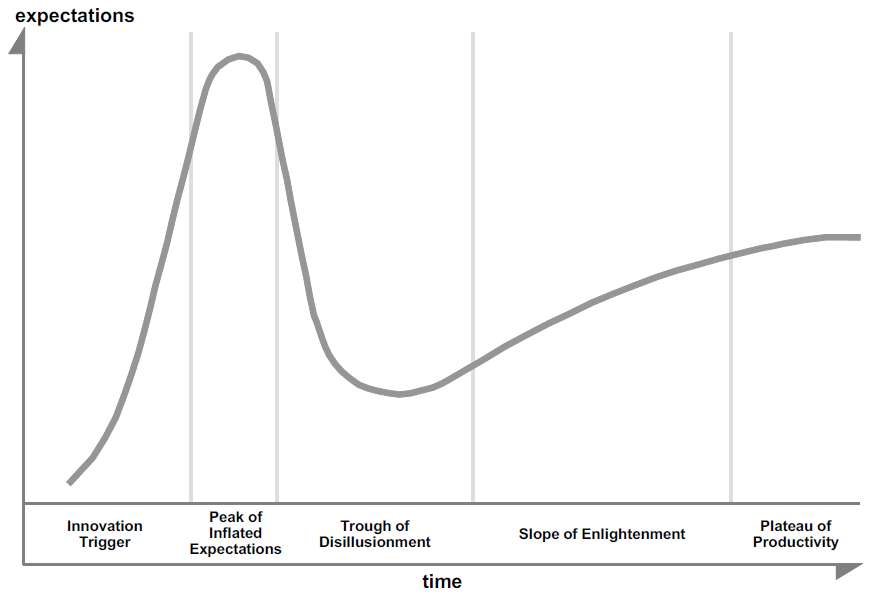
\includegraphics[width=0.9\linewidth]{img/ghc_raw}
	\caption*{\protect\fullciteNP<Quelle:>[S.~4]{Fenn2017}}
	\label{fig:ghc_raw}
\end{figure}

Anhand der Suchergebnisse wird jeder Technologie eine Matrix mit Suchmaschine, Jahr und Anzahl an Treffern zugeordnet. 

Der Betrachtungszeitraum für die Suche erstreckt sich über das Jahr des ersten Erscheinens einer der Technologien aus dem Abschnitt "`Peak of Inflated Expectations"' des "`Gartner Hype Cycle"' bis zum aktuellen Jahr. Das heißt, dass für die Ermittlung des Startjahres alle "`Hype Cycles"' der vergangenen Jahre in die Betrachtung einfließen, so lange mindestens eine der aktuellen Technologien im Abschnitt "`Peak of Inflated Expectations"' darin enthalten ist.

Alternativ kann das erstmalige Erscheinen einer Technologie im Abschnitt "`Innovation Trigger"' als Startzeitpunkt gewählt werden, sofern die Datenmenge im ersten Fall zu gering ausfällt.

Die ermittelte Verteilung der Mengen wird anschließend zunächst pro Suchmaschine und dann kumuliert betrachtet. Die dabei entstandene Kurve der Trefferanzahl über die Zeit wird dazu verwendet, die im Abschnitt "`Peak of Inflated Expectations"' erschienenen Technologien hinsichtlich des Trendverlaufes gegenüberzustellen.
	\section{Technologietrends in der praktizierenden Wirtschaft}

\subsection{Sicht auf Technologien}
Der Begriff Technologie lässt sich als eine spezielle Form des Wissens abstrahieren und entsteht dort, wo dieses Fachwissen Anwendung findet. Deshalb wird sie eher als ihre physikalische Ausprägung wie etwa in Form von Produkten und Systemen wahrgenommen.\footnote{\citeNP<Vgl.>[S.~6f]{Phaal2004}.} Da somit die Aneignung des theoretischen Wissens mit ihrer Implementierung in die Praxis zusammentrifft, ist die Entwicklung neuer Technologien mit verschiedenen Kosten verbunden.

Unternehmen bewegen sich deshalb in einem Spannungsfeld zwischen Investitionen in neue Technologien, um wettbewerbsfähig zu bleiben und optimaler Auslastung ihrer Ressourcenkapazitäten für bestehende Projekte. Denn die Erfolg versprechendste Technologie ist wirkungslos, wenn sie nicht zu einer geeigneten Zeit und mit richtigen Methoden eingesetzt wird.\footnote{\citeNP<Vgl.>[S.~518]{Dickinson2001}.}

Unter dem Begriff F\&E (Forschung und Entwicklung) werden die dafür notwendigen Maßnahmen bezeichnet, die strukturiert in einem Unternehmen gesteuert werden und die Gewinnung neuen Wissens im Bezug auf Technologien als Ziel verfolgen. Dazu werden Ressourcen des Unternehmens, wie etwa Mitarbeiter, monetäre Mittel etc. bereitgestellt, die zunächst einmal keinen unmittelbaren Ertrag herbeiführen, jedoch für die strategische Planung einen wichtigen Beitrag liefern. Ebenso werden Erkenntnisse über die unternehmenseigenen Stärken und Schwächen sowie externe Einflüsse des Marktes in Form von Chancen und Risiken gewonnen.\footnote{\citeNP<Vgl.>[S.~383f]{Jolly2003}.} Es handelt sich somit um eine Management-Tätigkeit, welche unter ständiger Berücksichtigung der Unternehmensziele die Gewinnung, Nutzung und den Schutz von Wissen anstrebt.

Nach Porter gehören F\&E deshalb zu den unterstützenden und nicht zu den primären Aktivitäten der Wertschöpfungskette. Dennoch hält er Technologien innerhalb eines Unternehmens für allgegenwärtig, also mehr oder weniger aller Aktivitäten inhärent. Sie erstrecken sich darüber hinaus auf Lieferanten, Kunden und die Vertriebspolitik, weshalb er hierfür den breiter gefassten Begriff Technologieentwicklung vorzieht.\footnote{\citeNP<Vgl.>[S.~36--42]{Porter1985}.}

Als Unterstützung für den Entscheidungsprozess, welche Technologien potentiell wertvoll im Sinne der Wettbewerbsfähigkeit sind und mit welchen Mitteln die Technologieentwicklung stattfinden sollte, wurden bereits in den 1980er-Jahren Konzepte für das Portfoliomanagement von Technologien entwickelt. Sie sollen die begrenzten Ressourcen eines Unternehmens ausgerichtet an Risiken, Erträgen und der Unternehmensstrategie effizient verteilen.\footnote{\citeNP<Vgl.>[S.~383f]{Jolly2003}.} 

Die wichtigsten Kriterien für die Auswahl der zu untersuchenden bzw. einzusetzenden Technologien ergeben sich aus der Auswertung beeinflussbarer und unbeeinflussbarer Faktoren. Bei den ersteren handelt es sich um firmenspezifische Merkmale sowie den Umgang mit der Wettbewerbssituation.\footnote{\citeNP<Vgl.>[S.~188]{Sinha2005}.} Die Fachkompetenz der Mitarbeiter kann beispielsweise durch Fortbildungen beeinflusst werden. Ebenso obliegt die Entscheidung über strategische Maßnahmen zur Konkurrenzabwehr in der eigenen Hand. Bei den unbeeinflussbaren Faktoren spielt vor allem die Marktsituation eine Rolle. Zum Beispiel ist in schnell wachsenden Marktsegmenten mit einer Vielzahl an Konkurrenten der Zugzwang Alleinstellungsmerkmale zu schaffen durch den Markt vorgegeben. Auch politische Entscheidungen, die direkt oder indirekt auf das eigene Handeln einwirken, liegen in der Regel nicht im Entscheidungsfreiraum eines Unternehmens.\footnote{\citeNP<Vgl.>[S.~188f]{Sinha2005}.}

Aus der Auswertung dieser Kriterien resultiert eine Tendenz, die genauere Prognosen für den optimalen Zeitpunkt des möglichen Einsatzes einer Technologie zulässt.\footnote{\citeNP<Vgl.>[S.~519]{Dickinson2001}.} Basierend darauf können im Hinblick auf potentielle Risiken und Gewinne Investitionen getätigt werden.\footnote{\citeNP<Vgl.>[S.~804]{Dolci2014}.}

\subsection{Einflussfaktoren auf Technologietrends}
Nach Worlton durchlaufen Technologietrends üblicherweise vier Phasen bis zur Marktreife: Erfindung, Innovation, Verschmelzung und Verbreitung. In der ersten Phase wird neues Wissen oder ein neues technisches Instrument generiert bzw. entwickelt. Die Erfindung allein ist dann allerdings in den meisten Fällen noch nicht marktreif, da der konkrete praktische Nutzen hier noch unbekannt ist. Dieser wird während der Innovationsphase durch Iterationen von Versuch und Irrtum in Ansätzen ermittelt. In Phase drei, der Verschmelzung, folgt erst der Durchbruch, indem verschiedene Technologien mit der neuen Erfindung kombiniert werden und ein neues Produkt bilden. Die vollständige Marktreife wird in Phase vier erreicht, wenn das neue Produkt in Stückzahlen produziert werden kann, die der Markt anfragt.\footnote{\citeNP<Vgl.>[S.~313]{Worlton1988}.}

In der wissenschaftlichen Literatur gibt es unterschiedliche Theorien über die treibende Kraft der Technologieentwicklung. Dabei sind zwei herrschende Meinungen festzustellen. Die erste besagt, dass Technologietrends durch äußere Einflüsse, wie den Verbraucher oder Anforderungen des Marktes geprägt werden. Demgegenüber lautet die zweite Annahme, dass der Anbieter im Rahmen seiner Kompetenzen und seines Einsatzes von F\&E Technologietrends ausschlaggebend vorgibt.\footnote{\citeNP<Vgl.>[S.~611]{Adner2001}.}

Adomavicius et al. zufolge ist eine monokausale Betrachtung für die Prognose von Technologietrends nicht zielführend, da sie die Ursachen trivialisiert, die Komplexität bei der Analyse aber nicht reduziert. Sie bevorzugen die Betrachtung von Technologien in einem Ökosystem, wo sie geboren werden, sich von da an stets gegenseitig beeinflussen, folglich einen evolutionären Entwicklungsprozess durchlaufen und wieder verschwinden können. Um die Komplexität der Technologielandschaft zu verringern, widmet er sich technischen Korrelationen zwischen verschiedenen Technologien, anstatt die äußeren Einflüsse Angebot und Nachfrage als alleinigen Impulsgeber zu verstehen.\footnote{\citeNP<Vgl.>[S.~785]{Adovamicius2016}.}

Um das Muster der Technologieentwicklung nachzuvollziehen, ist eine Unterteilung in folgende Rollen hilfreich:\footnote{\citeNP<Vgl.>[S.~786]{Adovamicius2016}.}
\begin{description}
	\item[Komponenten:] Teilstücke von Technologien, die kombiniert ein Produkt bilden.
	\item[Produkte:] Zusammengesetzte Komponenten, die mit dem Anwender interagieren.
	\item[Infrastruktur:] Unterstützen und erweitern die Nutzung eines Produktes.
\end{description}

In Tabelle \ref{tab:influence_path} sind die möglichen Kombinationen von Einflüssen vorhandener in Richtung zukünftiger Technologien abgebildet.

\begin{center}
\captionof{table}{Korrelation der Beeinflussung im technologischen Ökosystem}
\label{tab:influence_path}
\begin{tabulary}{\textwidth}{|L|C|C|C|}
	\hline
	 & zukünftige Komponente & zukünftiges Produkt & zukünftige Infrastruktur \\ 
	\hline 
	vorhandene Komponente &  &  &  \\ 
	\hline 
	vorhandenes Produkt &  &  &  \\ 
	\hline 
	vorhandene Infrastruktur &  &  &  \\ 
	\hline 
\end{tabulary}\par
\bigskip
\bigskip
Quelle: \citeNP<In Anlehnung an>[S.~785]{Adovamicius2016}.
\end{center}


%innovation process
%
%
%technology ecosystem
%Technology driven markets
%process-data-related, sensemaking
%
%Time to market
%
%Standards

\subsection{Informationsquellen von Unternehmern}
Gartner, Forrester, Aberdeen, and IDC

\subsection{Gartner’s Hype Cycle for Emerging Technologies}

\subsection{Schnittpunkte zur akademischen Forschung}
science-to-business
	\section{Technologietrends in der akademischen Forschung}
\subsection{Wissenschaftliche Fachzeitschriften}
Wissenschaftliche Publikationen sind für die Kommunikation und Verbreitung wissenschaftlicher Forschungsergebnisse von essenzieller Bedeutung und leisten einen wesentlichen Beitrag zum Erfolg des Forschenden.\footnote{\citeNP<Vgl.>[S.~417.]{Turbek2016}}

Sie werden hauptsächlich in regelmäßig erscheinenden wissenschaftlichen Fachzeitschriften veröffentlicht, in der Regel in englischer Sprache über einen Drittverlag und nicht der Universität des Autors.\footnote{\citeNP<Vgl.>[o. S.]{Bjork2009}} Zuvor wird ein \glqq Peer-Review\grqq~durch unabhängige Gutachter des gleichen Fachgebietes durchgeführt, bei dem die Qualität und Gültigkeit der Arbeit überprüft werden.\footnote{\citeNP<Vgl.>[S.~707.]{Thurner2011}}

Auch hinsichtlich Form, Umfang, Zitierweise und Schreibstil folgen sie meist bewährten Konventionen.\footnote{\citeNP<Vgl.>[o. S.]{Bjork2009}}

Einer Hochrechnung von \shortciteauthor{Jinha2010} zufolge wurden zwischen der ersten Veröffentlichung eines wissenschaftlichen Artikels im Jahre 1665 in Frankreich und dem Jahr der Studie 2009 insgesamt rund 50 Millionen Forschungsergebnisse nach einem \glqq Peer-Review\grqq~in wissenschaftlichen Artikeln publiziert. Die Verteilung der Publikationen über den analysierten Zeitraum zeigt dabei ein exponentielles Wachstum.\footnote{\citeNP<Vgl.>[S.~261f.]{Jinha2010}}

Im Zeitalter des Internets sind wissenschaftliche Publikationen meist in digitaler Form verfügbar, obgleich der überwiegende Anteil für die Allgemeinheit kostenpflichtig ist.\footnote{\citeNP<Vgl.>[o. S.]{Bjork2009}} Die Entwicklung von wissenschaftlichen Datenbanken schon in der frühen Phase des Internets zeigt, wie wichtig die Speicherung und Verbreitung von Forschungsergebnissen für die Wissenschaft ist.\footnote{\citeNP<Vgl.>[S.~338.]{Falagas2007}}

Sie bieten erweiterte Funktionen zur Suche und Bibliometrie von Artikeln, und werden daher bei der Literaturrecherche ausgiebig eingesetzt, um bereits existierende Forschungsergebnisse auszuwerten. \footnote{\citeNP<Vgl.>[S.~1320.]{Archambault2009}}

\subsection{Bedeutung von Publikationen für die Forschung}
Die Verbreitung von Wissen, das mittels akademischer Forschung gewonnenen wurde, erfolgt hauptsächlich über zwei Kanäle: Lehre und Publikationen in wissenschaftlichen Zeitschriften. Letzterer gewinnt dabei immer mehr an Bedeutung, da er vor allem für Forscher, die am Anfang ihrer Laufbahn stehen, bessere Möglichkeiten für ihre Karriere bietet.\footnote{\citeNP<Vgl.>[S.~322f.]{DeRond2005}}

Der Aphorismus \glqq Publish or Perish\grqq\footnote{Englisch sinngemäß für \glqq Publizieren oder Untergehen\grqq.} verdeutlicht den Druck, der auf Wissenschaftlern lastet, relevante Forschungsergebnisse in renommierten Fachzeitschriften zu veröffentlichen, um die nötige Aufmerksamkeit auf die eigenen Fähigkeiten zu lenken und damit die Karriereoptionen zu verbessern.\footnote{\citeNP<Vgl.>[S.~391.]{Clapham2005}}

Eine kontinuierliche Veröffentlichung von Forschungsergebnissen kann auch für Unternehmen nützlich sein, da Innovationen, die von Wettbewerbern parallel entwickelt und patentiert werden, rechtlich weiterhin nutzbar bleiben.\footnote{\citeNP<Vgl.>[S.~927.]{Parchomovsky2000}}

\subsection{Trends in der akademischen Forschung}
Forschungstrends in der wissenschaftlichen Fachliteratur können sowohl interne als auch externe Ursachen haben. Typische interne Ursachen sind neue Entdeckungen und wissenschaftliche Durchbrüche durch andere Forscher, die erhöhte Forschungspotentiale auslösen können. Externe Ursachen sind natürliche bzw. gesellschaftliche Ereignisse, die unabhängig von der Forschung eintreten und Wissenschaftler dazu anregen können, ein Thema aus neuen Perspektiven zu untersuchen.\footnote{\citeNP<Vgl.>[S.~359.]{Chen2006}}

Bei den internen Ursachen sind kontinuierliche Verbesserungen an bestehenden Technologien von revolutionär neuen Technologien zu unterscheiden.\footnote{\citeNP<Vgl.>[S.~114.]{Dotsika2017}} Letztere haben weitreichendere Auswirkungen auf das sozioökonomische System und werden in der Literatur oft als \glqq Emerging Technologies\grqq~bzw. \glqq Disruptive Technologies\grqq~bezeichnet.\footnote{\citeNP<Vgl.>[S.~285.]{Li2018}} Der Unterschied besteht in der anwendungsorientierten Reife der neuen Technologie. Bei einer \glqq Emerging Technology\grqq~muss der praktische Nutzen einer theoretischen Erkenntnis zunächst festgestellt werden. Die sog. \glqq Disruptive Technology\grqq~hat diese Phase bereits durch eine signifikante finanzielle oder technologische Verbesserung positiv gemeistert.\footnote{\citeNP<Vgl.>[S.~294.]{Li2018}}

Diese Art von Technologien haben einen potentiell stärkeren Effekt auf Forschungstrends in der Wissenschaft als solche, die auf Basis vorhandener Technologien mit marginalen Verbesserungen ausgestattet wurden.

\shortciteauthor{Price1965} zufolge kann ein Muster für Forschungsschwerpunkte zu einem bestimmten Thema beobachtet werden. Neue wissenschaftliche Artikel beziehen sich demnach eher auf die aktuellsten Publikationen als auf deren Vorgänger. Im Umkehrschluss bedeutet das, dass die meist zitierten Artikel gleichzeitig auch die aktuellsten sind.\footnote{\citeNP<Vgl.>[S.~512f.]{Price1965}} Dieser Effekt gibt eine gute Erklärung für das bekannte Phänomen, dass Artikel wenige Jahre nach ihrer Veröffentlichung als veraltet gelten.\footnote{\citeNP<Vgl.>[S.~360.]{Chen2006}}

\subsection{Schnittstellen mit der praktizierenden Wirtschaft}
Da die öffentlichen Mittel für die akademische Forschung heute nicht wesentlich zunehmen, wird die industrielle Zusammenarbeit von vielen Wissenschaftlern als eine Strategie angesehen, um mehr finanzielle Unterstützung für ihre Forschung zu erhalten.\footnote{\citeNP<Vgl.>[S.~86.]{Calvert2003}}

	\section{Methodische Vorgehensweise}
\subsection{Datenerhebung}
Für die Gegenüberstellung der Technologietrends in der akademischen Forschung und praktizierenden Wirtschaft werden, wie bereits in Abschnitt \ref{sec:method} erwähnt, zwei Arten von Quellen herangezogen.

Der \glqq Gartner Hype Cycle for Emerging Technologies\grqq~repräsentiert als marktführendes Unternehmen für Technologieprognosen den Part der praktizierenden Wirtschaft. Dabei dienen die Technologien im Bereich der \glqq Peak of Inflated Expectations\grqq~in vorliegender Gewichtung als Datenbasis für die Analyse.

Demgegenüber wird die Datenbasis der akademischen Forschung aus Abfragen in relevanten Literaturdatenbanken erhoben. 

\subsection{Operationalisierung der Daten}
\subsection{Methodik der Analyse}
	\renewcommand{\refname}{Literaturverzeichnis}
	\pagenumbering{roman}
	\lhead{}
	\linespread{1}
	\bibliography{lit}
	\newpage
\fancyhead[C]{\thepage}
\pagenumbering{gobble} % Keine Seitenzahlen mehr

%-----------------------------------
% Ehrenwörtliche Erklärung
%-----------------------------------
\section*{Ehrenwörtliche Erklärung}
Hiermit versichere ich, dass die vorliegende Arbeit von mir selbstständig und ohne unerlaubte Hilfe angefertigt worden ist, insbesondere dass ich alle Stellen, die wörtlich oder annähernd wörtlich aus Veröffentlichungen entnommen sind, durch Zitate als solche gekennzeichnet habe. Ich versichere auch, dass die von mir eingereichte schriftliche Version mit der digitalen Version übereinstimmt. Weiterhin erkläre ich, dass die Arbeit in gleicher oder ähnlicher Form noch keiner Prüfungsbehörde / Prüfungsstelle vorgelegen hat. Ich erkläre mich damit einverstanden, dass die Arbeit der Öffentlichkeit zugänglich gemacht wird. Ich erkläre mich damit einverstanden, dass die Digitalversion dieser Arbeit zwecks Plagiatsprüfung auf die Server externer Anbieter hochgeladen werden darf. Die Plagiatsprüfung stellt keine Zurverfügungstellung für die Öffentlichkeit dar.


\vspace{5cm}

\begin{table}[h]
	\centering
	\begin{tabular*}{\textwidth}{c @{\extracolsep{\fill}} ccccc}
		Gelsenkirchen, \today
		&
		%PLACE YOUR SCANNED SIGNATURE INSIDE YOUR PICTURE DIRECTORY. CALL IT unterschrift.jpg
%		
\includegraphics[width=0.35\textwidth]{img/unterschrift}\vspace*{-0.35cm}
		\\
		\rule[0.5ex]{12em}{0.55pt} & \rule[0.5ex]{12em}{0.55pt} \\
		(Ort, Datum) & (Eigenhändige Unterschrift)
		\\
	\end{tabular*} \\
\end{table}

\end{document}